\section{Pendahuluan}
\subsection{Latar Belakang}
Jaringan komputer memiliki peran yang sangat penting yang melengkapi berbagai keperluan pada lingkup pendidikan, bisnis, maupun pemerintahan. Hal tersebut bertujuan untuk penyaluran data komunikasi yang efisien dan cepat. Perancangan dserta pengelolaan jaringan yang baik menjadi aspek penting.

Setiap instansi membutuhkan jaringan komputer yang dapat menghubungkan semua perangkat yang mereka miliki agar dapat saling mendapatkan dan mengirim data. Tidak serta-merta semua perangkat milik instansi dihubungkan dengan masing-masing satu kabel untuk setiap hubungan antar perangkat. Oleh karena itu, terdapat struktur jaringan yang dapat membantu "mengarahkan" data antar perangkat dengan lebih terstruktur dan efisien.

\subsection{Dasar Teori}
Crimping merupakan sebuah proses untuk menyambung kabel UTP dengan konetor RJ45. Kabel UTP terdiri dari 4 warna dan 4 warna strip, dimana kabel warna strip pasangan dari kabel warna, sehingga dalam satu kabel UTP terdapat 8 kabel. Warna dalam kabel UTP dapat dikonfigurasi menjadi dua, yaitu: T-568A dan T-568B. Koneksi antar konektor RJ45 dapat berupa : Straight-through, digunakan untuk menghubungkan ke kedua perangkat yang berbeda jenis. contohnya, komputer ke router, konfigurasi T-568A ke/dari T-568A. Crossover, digunakan untuk menghubungkan perangkat yang sejenis contohnya, komputer ke komputer, konfigurasi T-568A ke/dari T-568B.

IPv4 atau Internet Protocol version 4 digunakan untuk identifikasi dan mengatur addressing perangkat dalam sebuah jaringan komputer berbasis TCP/IP. IPv4 memiliki panjang address sebesar 32bit, yang dibagi menjadi empat oktet dimana masing-masing oktet sepanjang 8 bit. Pada umumnya IPv4 ditulis dalam decimal. Alamat IPv4 terdiri dari dua bagian yaitu, Network ID yang menunjukan id jaringan, dan Host ID yang menunjukan id host dalam jaringan, misal: Alamat IP adalah 192.168.1.10/24, maka Network ID adalah 192.168.1 dan Host ID adalah .10. Karena Subnet pada CIDR /24 dimana 24 bit pertama adalah Network ID dan 8 bit sisa adalah Host ID. Subnetting digunakan untuk membagi satu jaringan besar menjadi sub-jaringan. Digunakan untuk mengoptimalkan pengguanaan address IP dan keamanan.

%===========================================================%
\section{Tugas Pendahuluan}
\begin{enumerate}
	\item Jaringan utama akan berada pada address 192.168.100.0/24, semua IP pada departemen yang tercakup akan berada pada range 192.168.100.0 - 192.168.100.255. Akan dibuat 4 subnet berdasarkan masing-masing departemen. Departemen R\&D membutuhkan 100 perangkat sehingga yang paling memungkinkan adalah menggunakan CIDR /25, karena dapat menampung 126 usable IP dalam subnet tersebut, sehingga range IP departemen tersebut adalah 192.168.100.2 - 192.168.100.127. Departemen Produksi membutuhkan 50 perangkat dapat menggunakan CIDR /26, karena dapat menampung 62 usable IP sehingga range IP departemen tersebut adalah 192.168.100.130 - 192.168.100.191. Departemen Administrasi membutuhkan 20 perangkat dapat menggunakan CIDR /27, karena dapat menapung 30 usable IP sehingga range IP departemen tersebut adalah 192.168.100.194 - 192.168.100.223. Departemen Keuangan membutuhkan 10 perangkat dapat menggunakan CIDR /28, karena dapat menampung 14 usable IP sehingga range IP departemen tersebut adalah 192.168.100.226 - 192.168.100.234. Semua usable IP dikurang satu untuk address gateway router masing-masing departemen.
	\item Topology jaringan
    \begin{figure}[H]
	    \centering
	    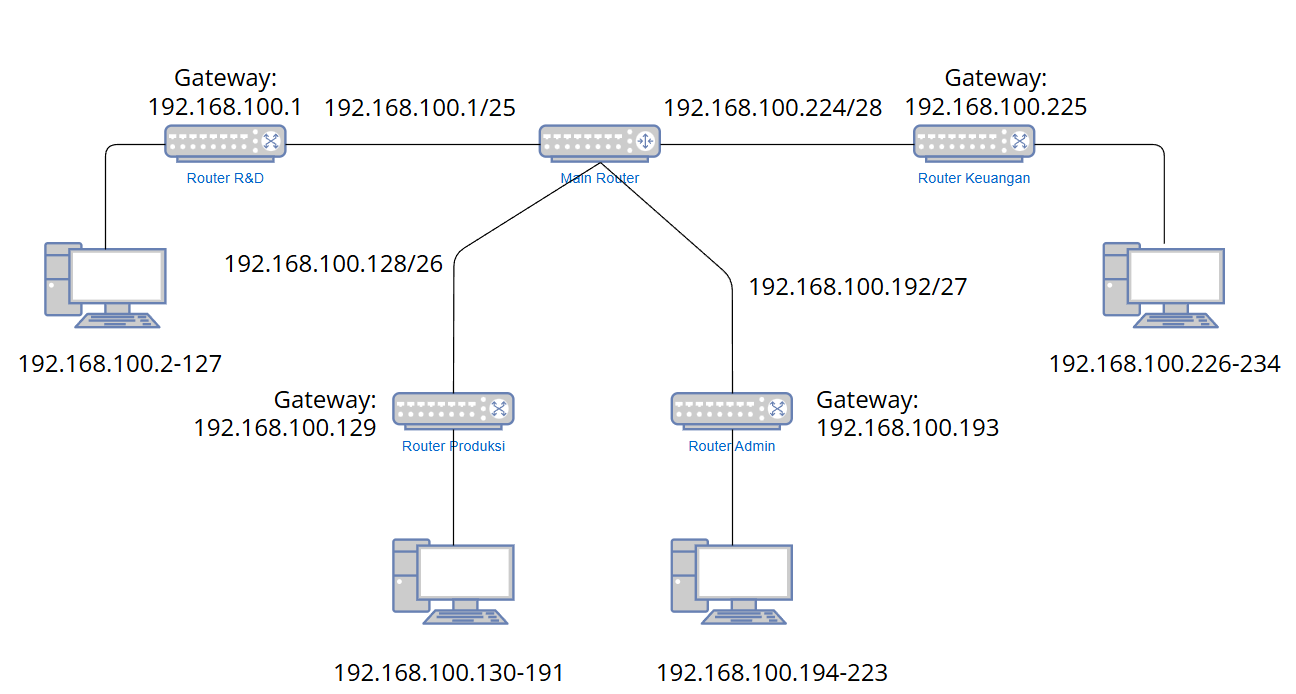
\includegraphics[width=1\linewidth]{Cover/img/topologi.png}
	    \caption{Topology}
	    \label{fig:enter-label}
	\end{figure}
		\item  \hspace{2cm}
        \begin{tabular}{|c|c|c|c|c|}
        \hline
        Destination & Netmask & Gateway & Interface & Keterangan \\
        \hline
        192.168.100.0 & /25    & 192.168.100.1    & Direct    & e0    \\
        \hline
        192.168.100.128 & /26    & 192.168.100.129    & Direct    & e1    \\
        \hline
        192.168.100.192 & /27    & 192.168.100.193    & Direct    & e2   \\
        \hline
        192.168.100.224 & /28    & 192.168.100.225    & Direct    & e3    \\
        \hline
        \end{tabular}

    \item Jenis routing yang cocok untuk perusahaan ini adalah static routing. Hal ini dikarenakan topology yang digunakan sederhana dan jelas. Subnet yang dibutuhkan perushaan juga sedikit hanya empat. Keuntungan dari static routing adalah lebih mudah dikelola dan tidak memakan resource yang banyak.
        
\end{enumerate}